\documentclass{beamer}
\usetheme{AnnArbor}
\usepackage[letterpaper, margin=1in]{geometry}
\usepackage{graphicx}
\usepackage{hyperref}
\usepackage{mdframed}
\usepackage{xcolor}

\setbeamersize{text margin left=16mm, text margin right=16mm}
\setbeamercolor{normal text}{fg=black, bg=white}

\setbeamercolor{frametitle}{bg=cyan!30}
\setbeamerfont{frametitle}{size=\LARGE}
\setbeamerfont{normal text}{size=\Large}
\setbeamerfont{itemize/enumerate body}{size=\Large}

\title{Restaurant Management System}
\institute{SVECW}
\date{\today}

\begin{document}

\begin{frame}
  \begin{center}
    
\includegraphics[width=2cm]{logo.png}
  \end{center}

  \begin{center}
    \textbf{\large \colorbox{yellow!20}{Shri Vishnu Engineering College for Women}}
  \end{center}

  \begin{center}
    \textbf{\large\colorbox{purple!20}{Project Name: Restaurant Management System}}
  \end{center}

  \begin{flushleft}
    \textbf{\large\colorbox{blue!20}{Team Members:}}
  \end{flushleft}

  \begin{itemize}
          \item{\small\textbf {22B01A1299 - M.Nikitha(Developer,Git)}}
          \item{\small\textbf {22B01A12A0 - M.Kalyani(Developer)}}
           \item{\small\textbf {22B01A1281 - K.Vaishnavi(Developer)}}
          \item{\small\textbf {22B01A12B8 - P.Lekha Ravali(Latex,Developer)}}
          \item{\small\textbf {22B01A12C4 - P.Devi Priyanka(Developer)}}
  \end{itemize}
\end{frame}

\begin{frame}
  \frametitle{DESCRIPTION}


\textbf{\large {The restaurant management system is designed for:}}
      \begin{itemize}
    \item Employee Management
     \item Menu creation and Management
      \item Sales Tracking
      \item Billing process
  \end{itemize}
\end{frame}

\begin{frame}
  \frametitle{ABSTRACT}

  \begin{itemize} \item The Restaurant Management System designed to streamline and optimize various aspects of restaurant operations,including Employee Management, Menu Creation, Sales tracking, Billing Process and User Authentication.
  \end{itemize}
\end{frame}




\begin{frame}
   \frametitle{DATA FLOW DIAGRAM}
   \begin{figure}
      \centering
      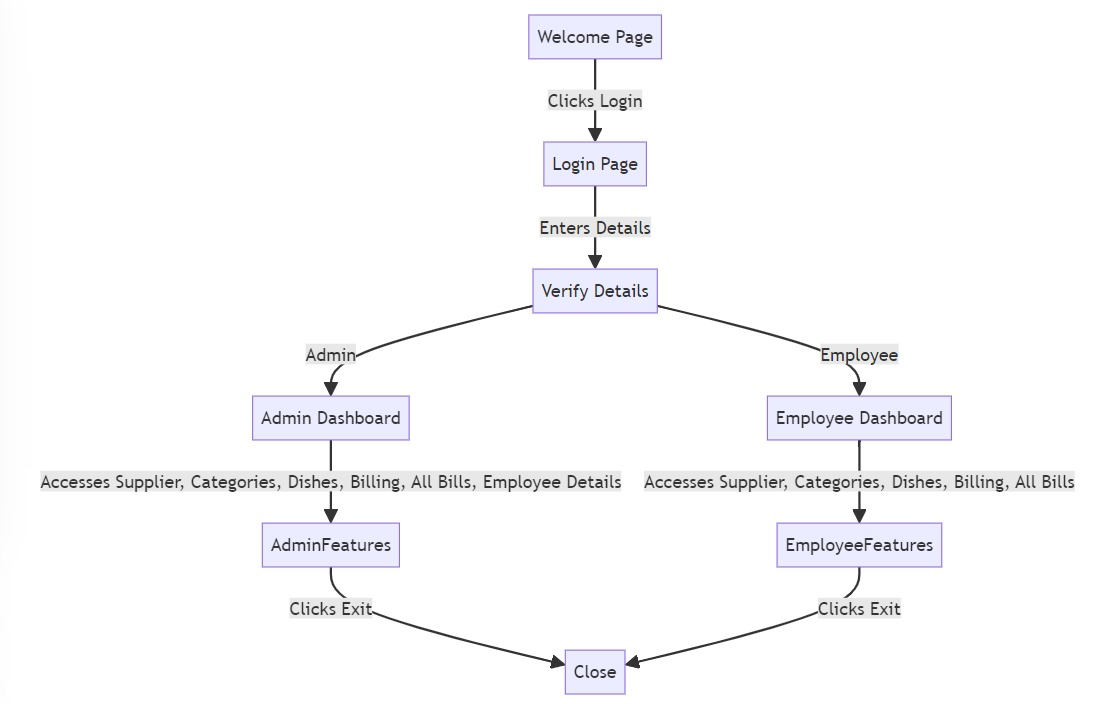
\includegraphics[width=1.1\linewidth]{dataflow.jpg}
    \end{figure}
\end{frame}  

\begin{frame}
  \frametitle{Home Page}
  \begin{figure}
    \centering
    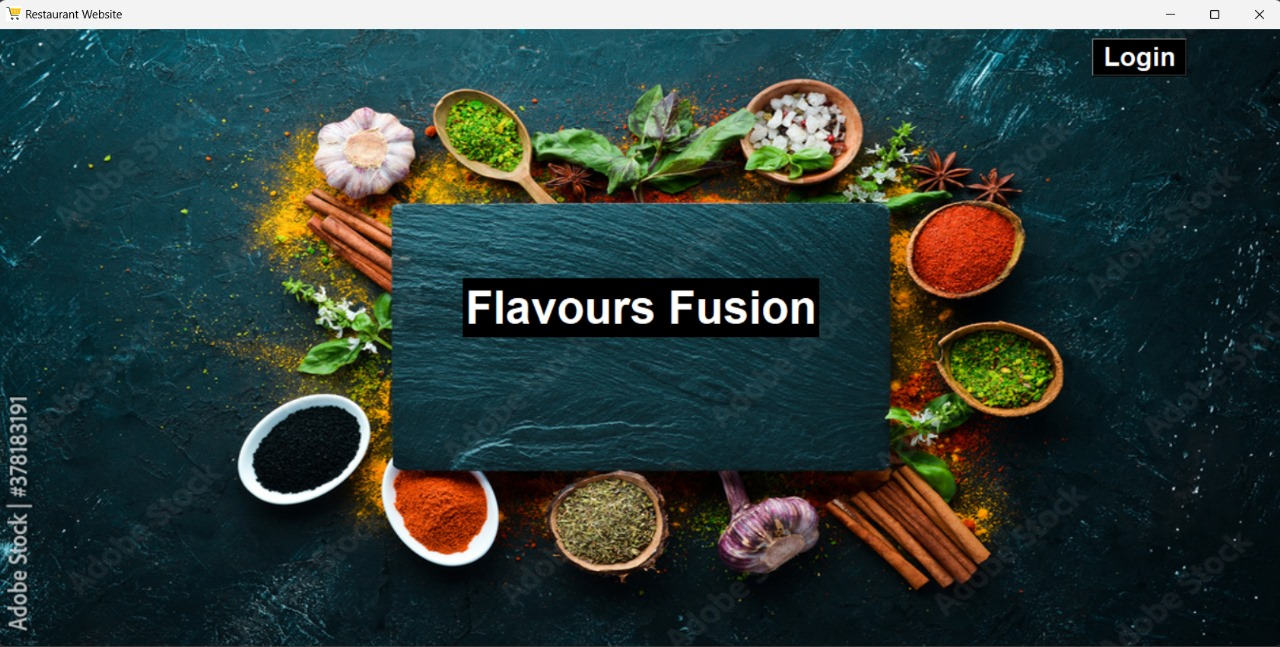
\includegraphics[width=1.0\linewidth]{homepage.jpg} 
  \end{figure}
\end{frame}


\begin{frame}
  \frametitle{LOGIN PAGE}
  \begin{figure}
    \centering
    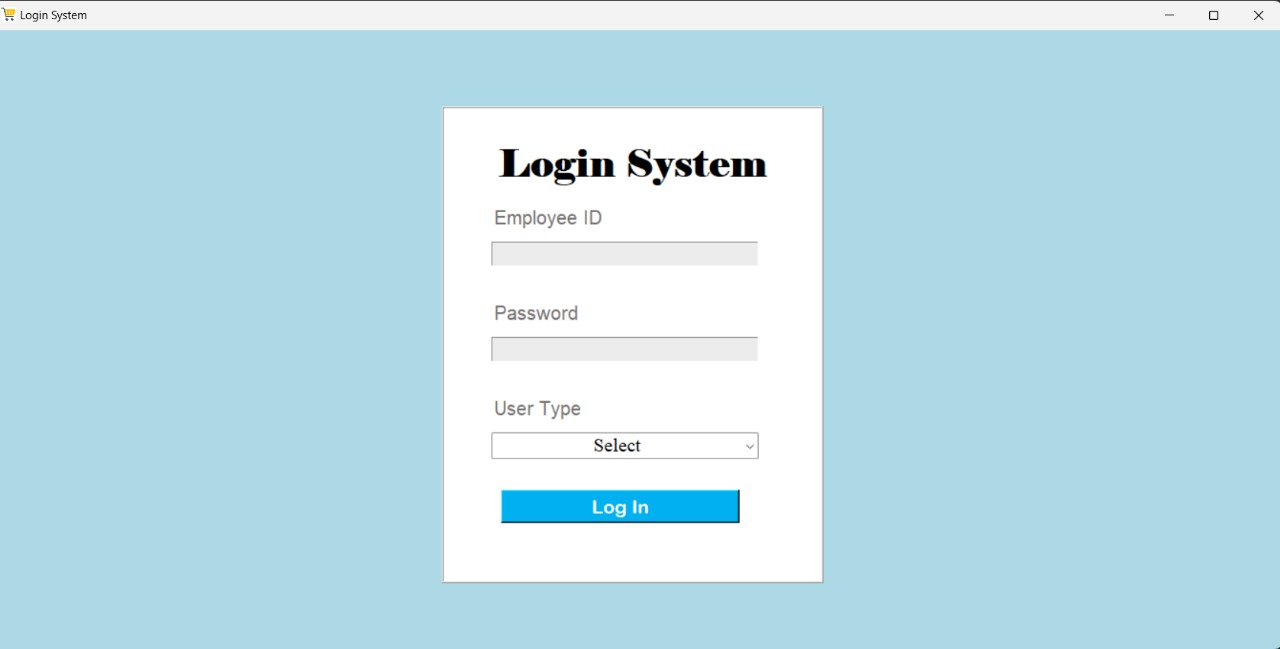
\includegraphics[width=1.0\textwidth]{loginpage.jpg}
  \end{figure}
\end{frame}

\begin{frame}
  \frametitle{ADMIN DASHBOARD}
  \begin{figure}
    \centering
    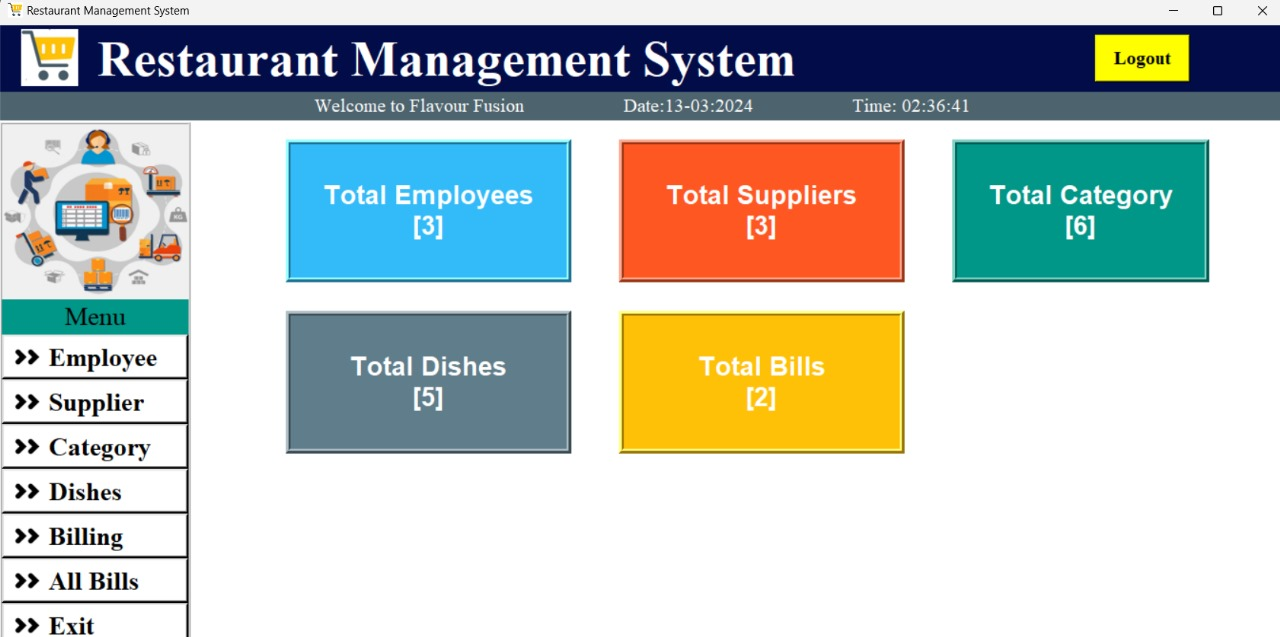
\includegraphics[width=1\linewidth]{admindashboard.jpg} 
  \end{figure}
\end{frame}


\begin{frame}
  \frametitle{EMPLOYEE DETAILS PAGE}
  \begin{figure}
    \centering
    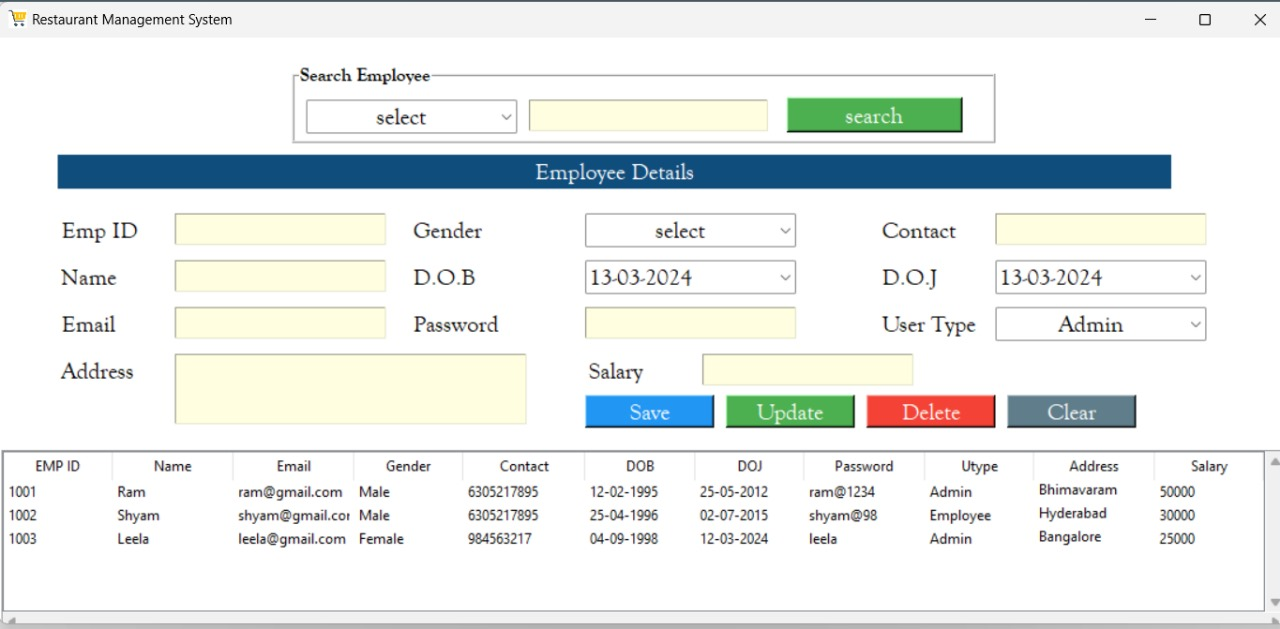
\includegraphics[width=1.0\linewidth]{employeedetailspage.jpg} 
  \end{figure}
\end{frame}


\begin{frame}
  \frametitle{Employee Dashboard}
  \begin{figure}
    \centering
    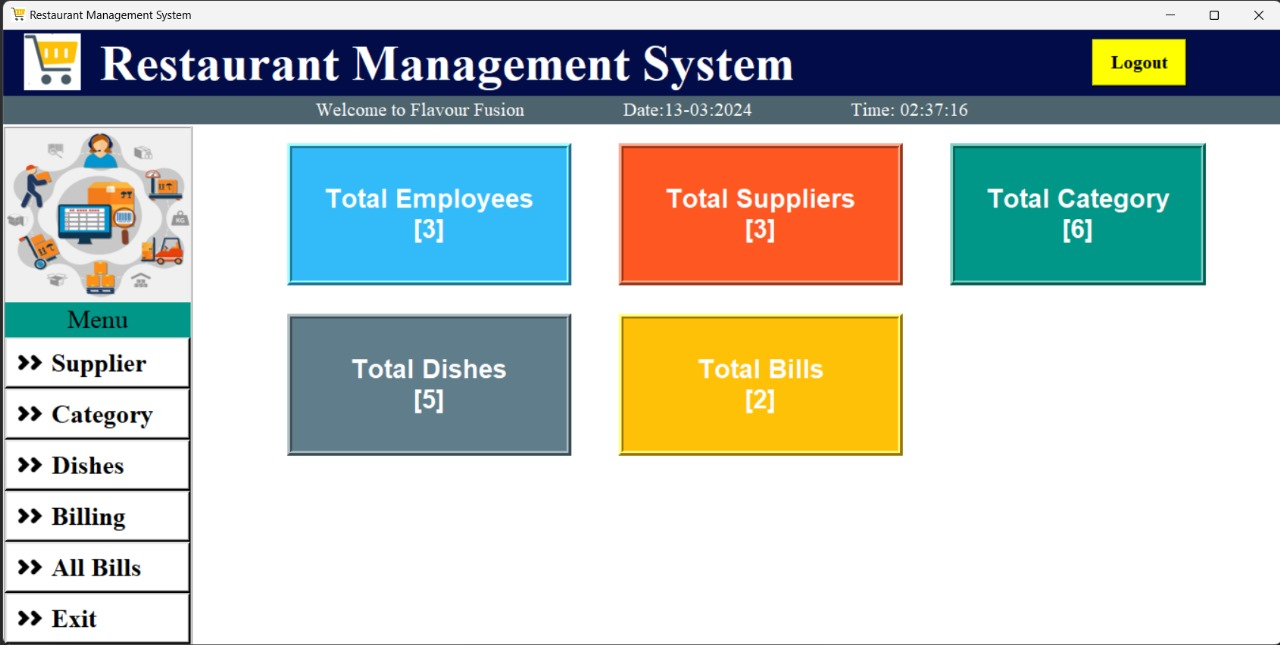
\includegraphics[width=1.0\linewidth]{employeedashboard.jpg} 
  \end{figure}
\end{frame}

\begin{frame}
  \frametitle{SUPPLIERS PAGE}
  \begin{figure}
    \centering
    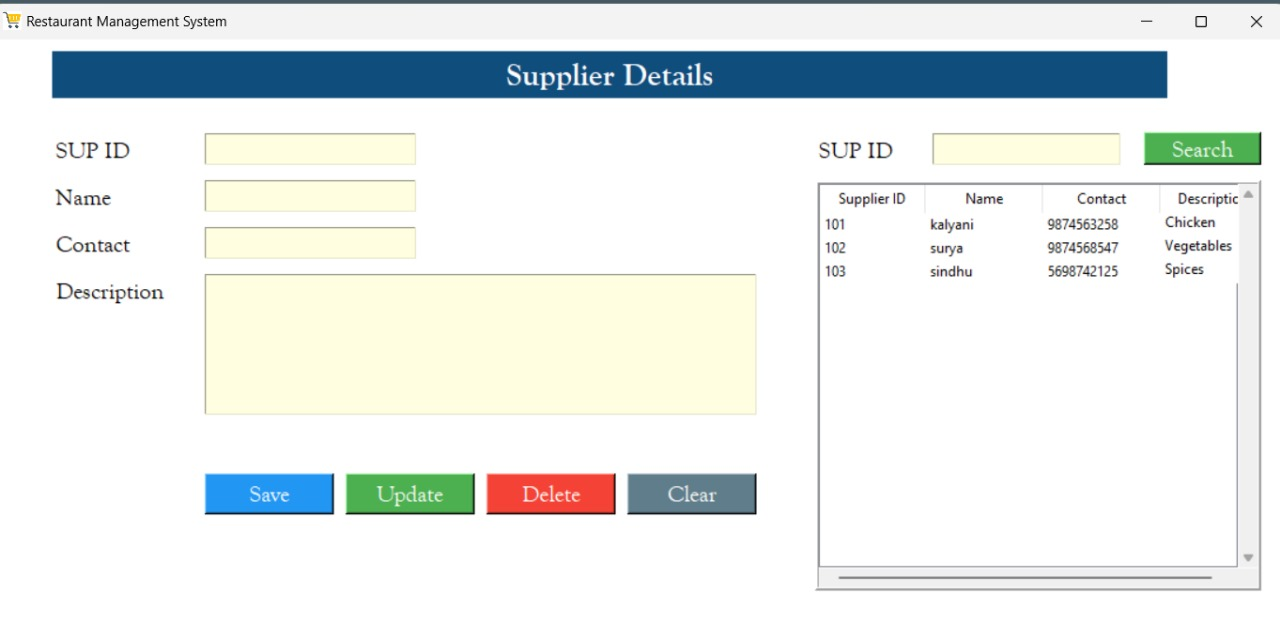
\includegraphics[width=1.0\linewidth]{supplierspage.jpg} 
  \end{figure}
\end{frame}

\begin{frame}
  \frametitle{CATEGORY PAGE}
  \begin{figure}
    \centering
    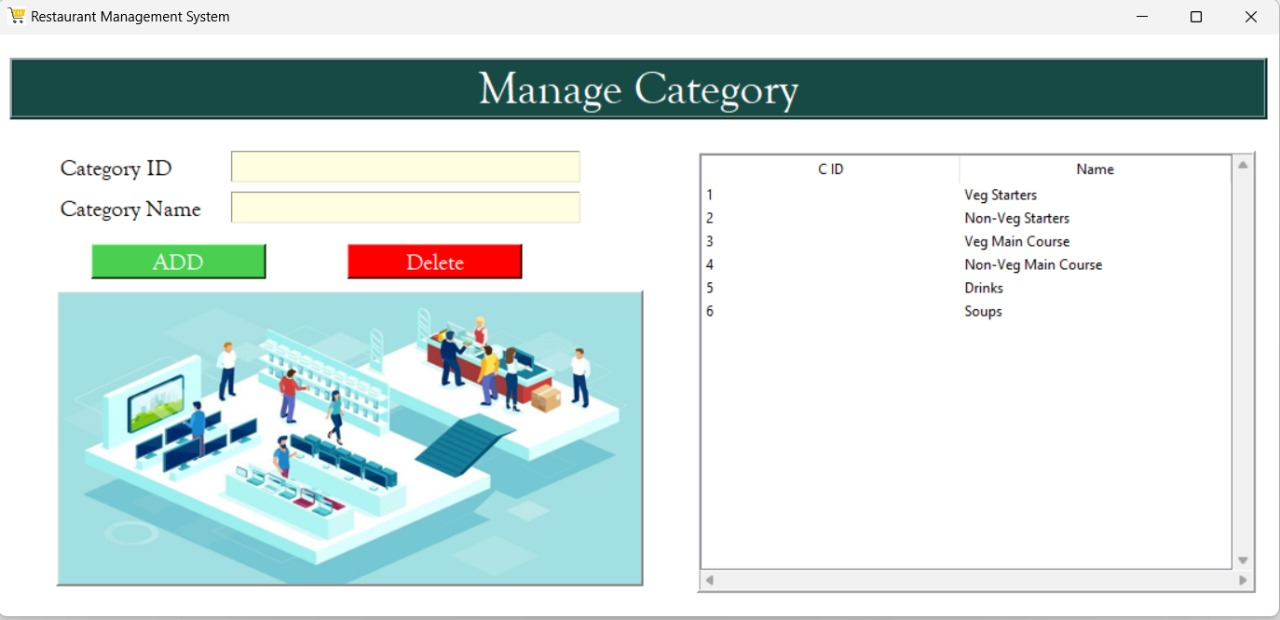
\includegraphics[width=1.0\linewidth]{categorypage.jpg} 
  \end{figure}
\end{frame}


\begin{frame}
  \frametitle{Dishes Page}
  \begin{figure}
    \centering
    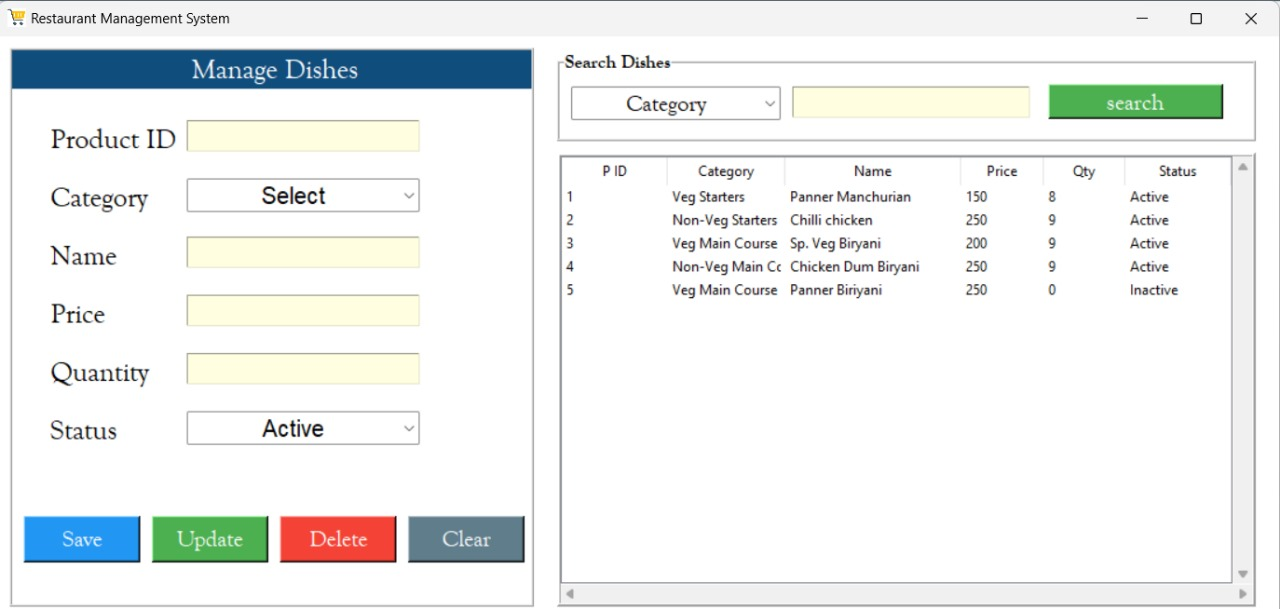
\includegraphics[width=1.0\linewidth]{dishespage.jpg} 
  \end{figure}
\end{frame}



\begin{frame}
  \frametitle{Billing page}
  \begin{figure}
    \centering
    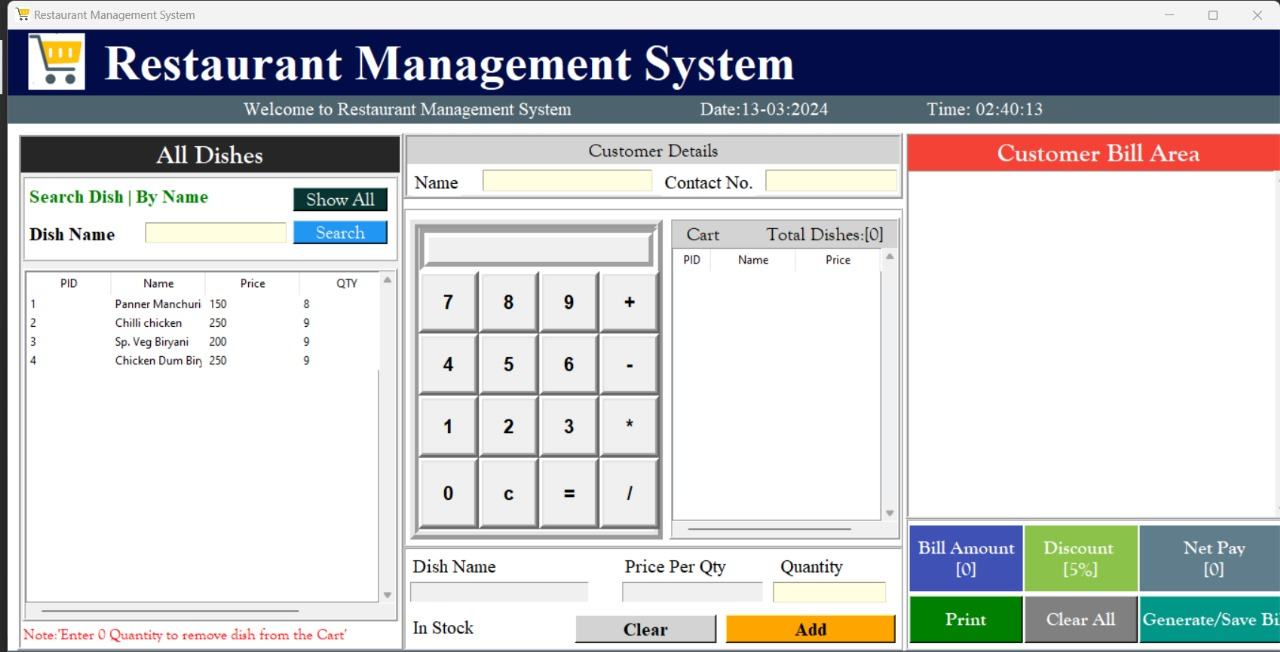
\includegraphics[width=1.0\linewidth]{billingpage.jpg} 
  \end{figure}
\end{frame}


\begin{frame}
  \frametitle{ALL BILLS PAGE}
  \begin{figure}
    \centering
    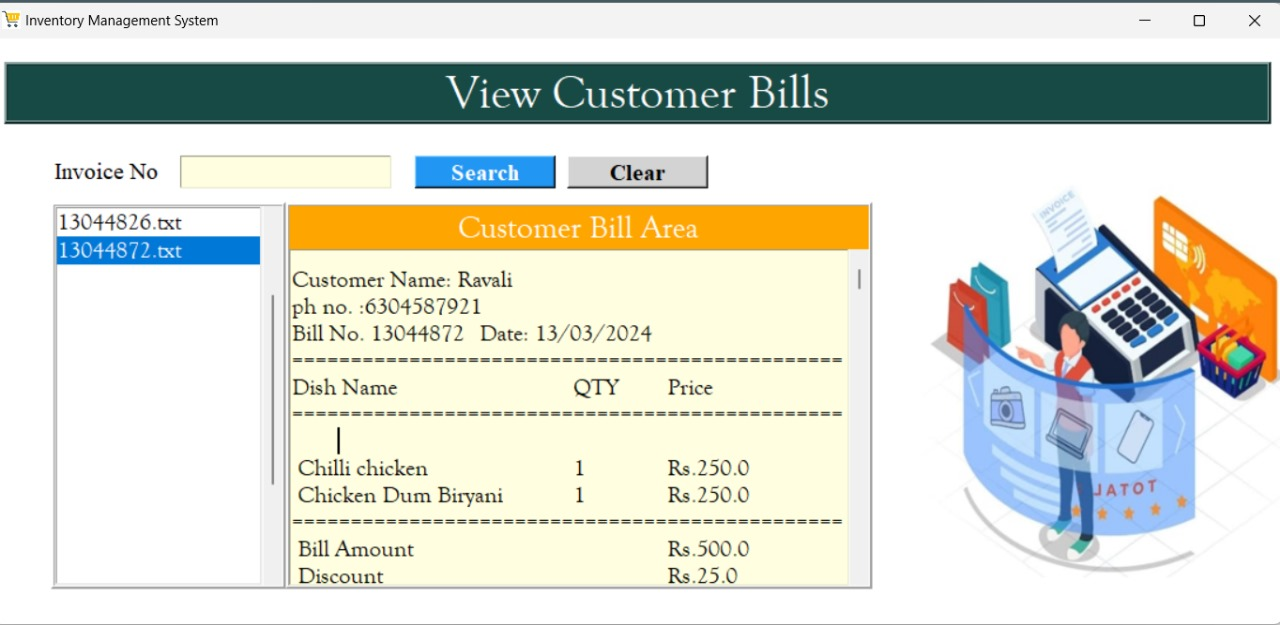
\includegraphics[width=1.0\linewidth]{allbillspage.jpg} 
  \end{figure}
\end{frame}

\begin{frame}
    \frametitle{BIBLIOGRAPHY}
     \begin{itemize}
        \small\item Building Modern GUI's with TKInter and Python: Building user friendly GUI applications with ease by \textbf{SaurabhChandrakar}\\[10pt]
        
        \small\item TKInter GUI application development blueprints build nine projects by working with widgets, geometry management, event handling, and  more by \textbf{BhaskarChaudhary}\\[10pt]
        \item\href{https://www.researchgate.net/publication/340938646_Databases_with_SQlite_using_Python_Tutorial}{\textcolor{blue}{Database with SQLite using Python Tutorial}}.
        \end{itemize}

\end{frame}

\end{document}